%!TEX root = ../luanvan.tex
\chapter{Kết quả thực nghiệm}
\section{Mạng blockchain}

{\color{red} Todo: phần này nên chia làm 2 subsection: subsection đầu tiên mô tả mô trường, công cụ, nền tảng để xây dựng mạng. Subsection tiếp theo mô tả các bước xây dựng mạng và kết quả đạt được.}

Mạng Blockchain được cài đặt  trên máy tính cá nhân có cấu hình như sau:
\begin{itemize}
\item CPU: Intel(R) Core(TM) i3-10100F 3.00 GHz
\item RAM: 16 GB
\item Hard Disk: 120 GB NVME SSD
\end{itemize}

Máy tính được thiết lập theo các bước sau:
\begin{enumerate}
\item Mở Visual Studio Code 
\item Tìm extension IBM Blockchain Flatform, chọn cài đặt.
\end{enumerate}
Mạng Blockchain Fabric hoạt động như hình \ref{fig:ide_start}, blockchain thử nghiệm chaincode gồm có tổ chức Org1, peer, CA, Order, OrdererMSP, Org1MSP

\begin{figure}[htbp]
\centering
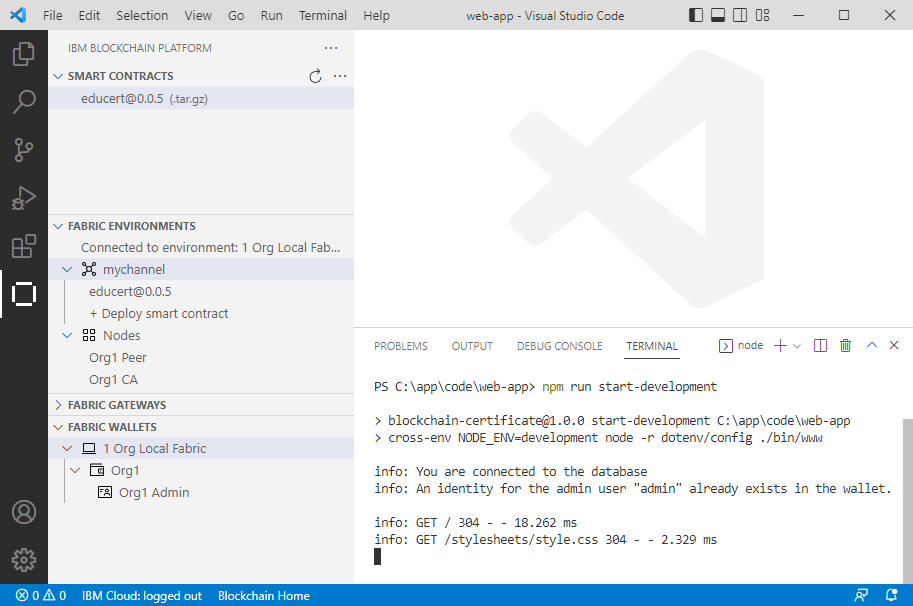
\includegraphics[width=.9\linewidth]{img/ide_start.PNG}
\caption{Chương trình Visual Studio Code}
\label{fig:ide_start}
\end{figure}

\section{Ứng dụng Web}

{\color{red} Todo: Cần bổ sung diễn giải ý nghĩa của các giao điện màn hình theo các bước của quy trình tổng thể ở chương 3.

Không thể trình bày như thế này: chỉ chụp màn hình đưa vào là xong đc, phải mô tả, diễn giải thông tin, chức năng, ý nghĩa, sực khác biệt giữa có và không có Blockchain ở từng bước này!
}

Giao diện ứng dụng web hoạt động tại địa chỉ http://localhost:3000/ như hình \ref{fig:main_vbcc}. 

\begin{figure}[H]
\centering
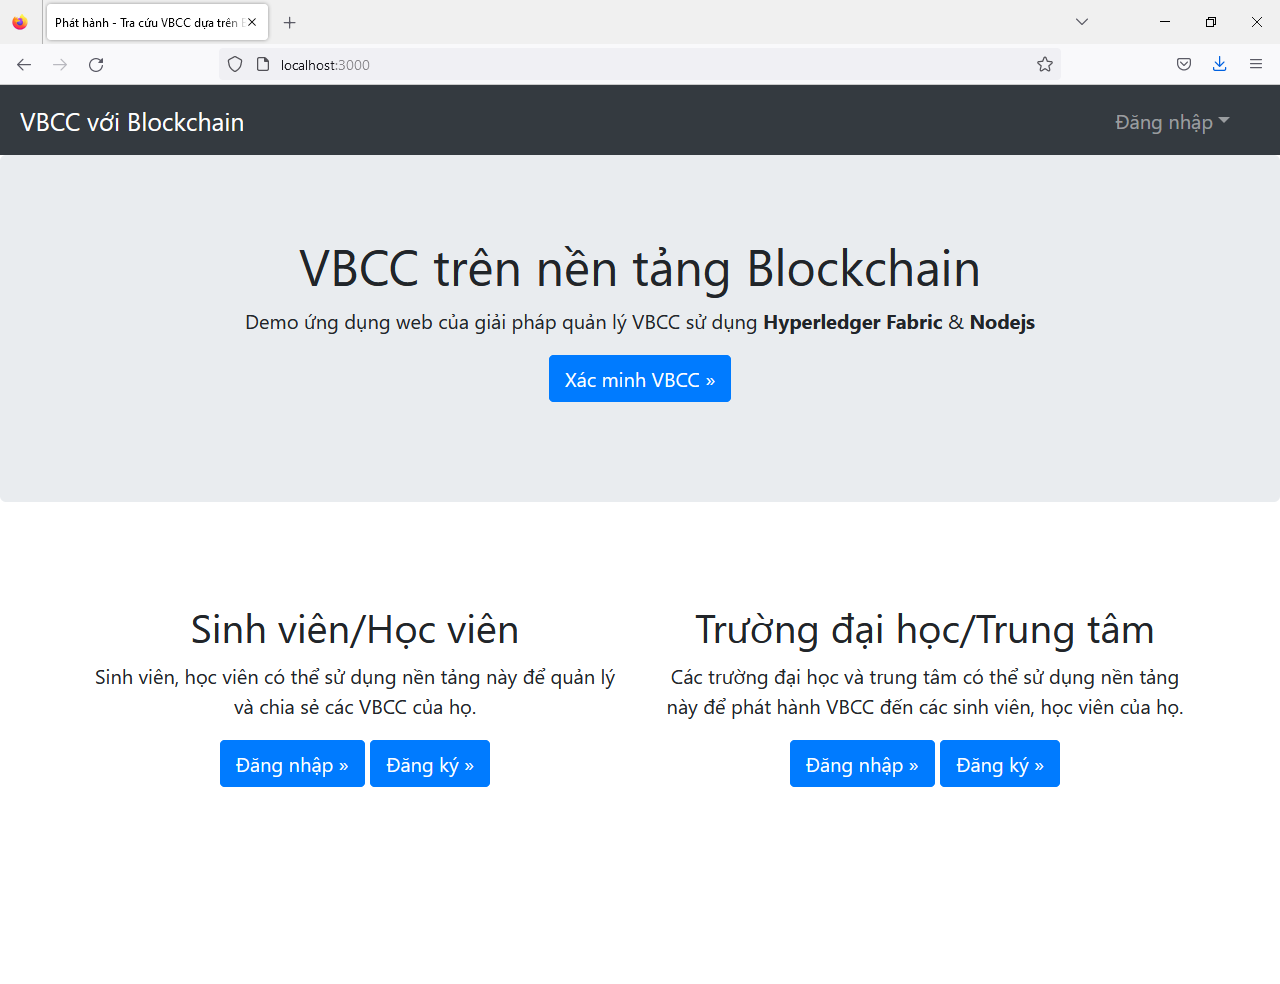
\includegraphics[width=.9\linewidth]{img/main_vbcc.png}
\caption{Giao diện hệ thống}
\label{fig:main_vbcc}
\end{figure}

Trường, trung tâm có chức năng

\begin{figure}[H]
\centering
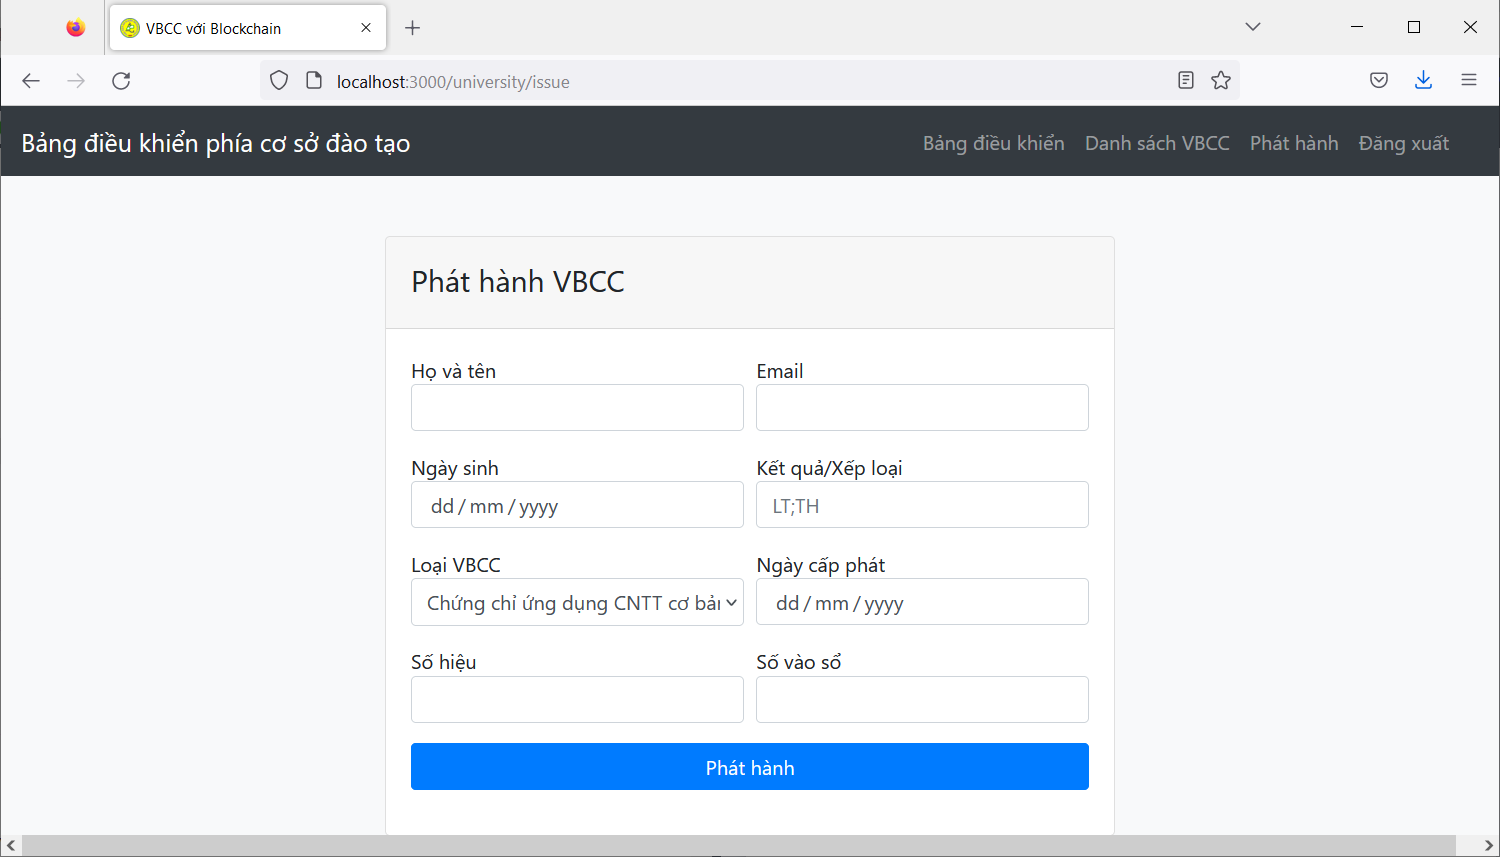
\includegraphics[width=.9\linewidth]{img/tt_phathanh.PNG}
\caption{Màn hình cấp VBCC cho sinh viên}
\label{fig:tt_phathanh}
\end{figure}

\begin{figure}[H]
\centering
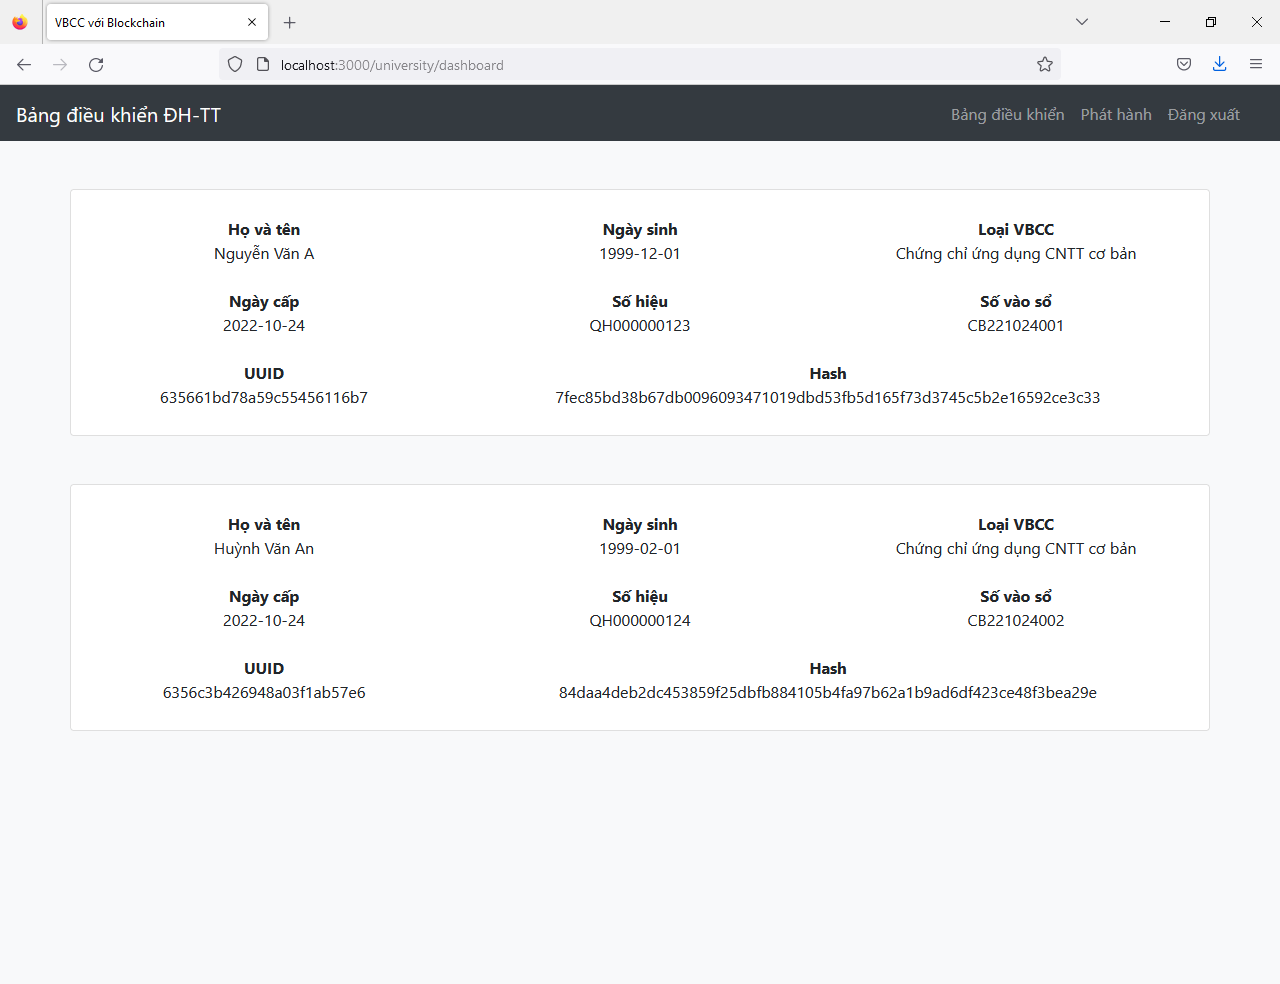
\includegraphics[width=.9\linewidth]{img/tt_dacap.PNG}
\caption{Màn hình xem các VBCC đã cấp}
\label{fig:tt_dacap}
\end{figure}


Sinh viên, học viên có chức năng

\begin{figure}[H]
\centering
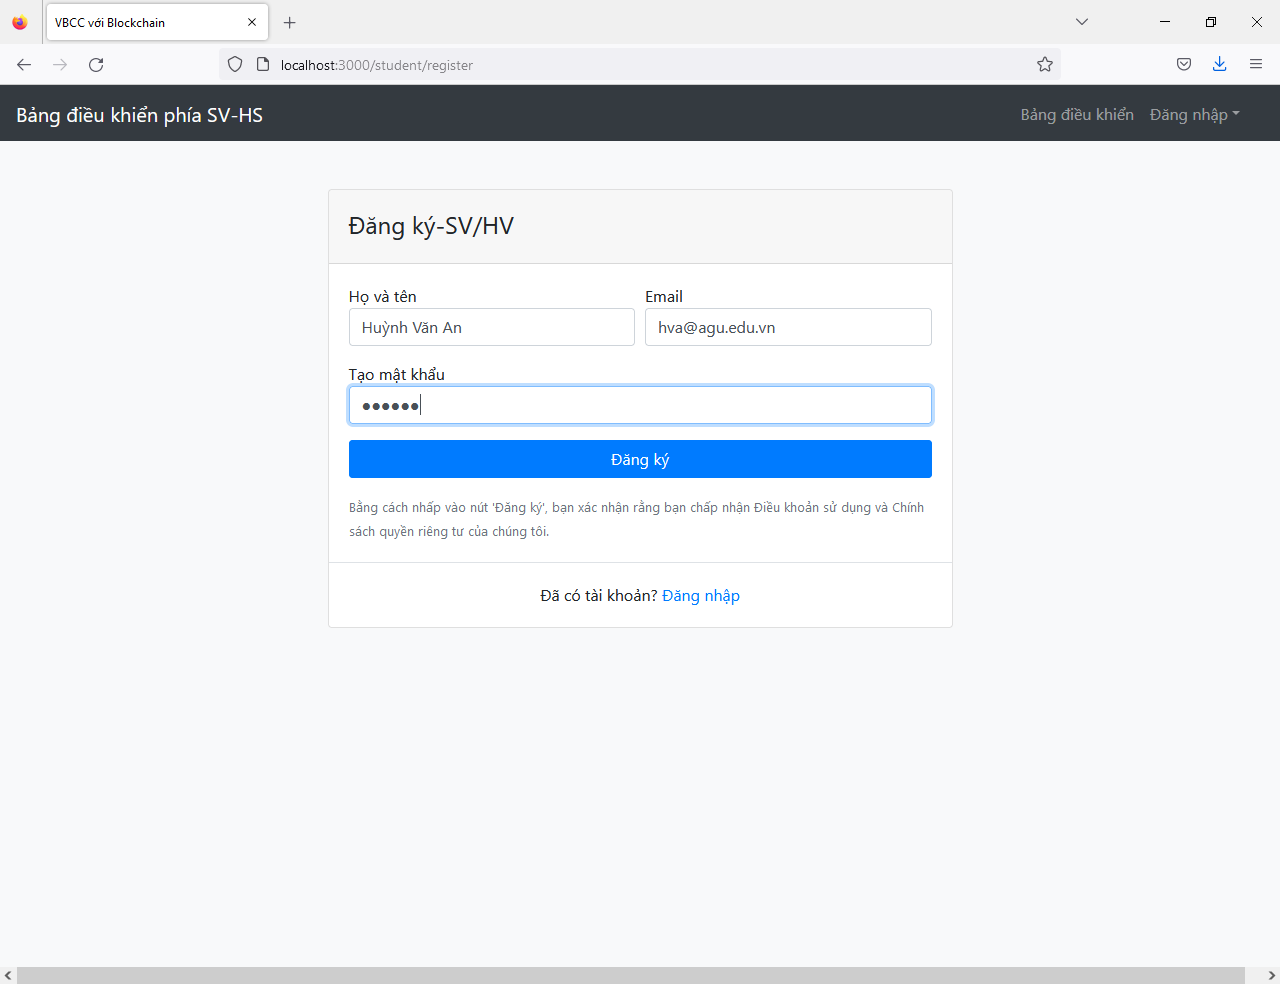
\includegraphics[width=.9\linewidth]{img/std_new.PNG}
\caption{Màn hình đăng ký tài khoản}
\label{fig:std_new}
\end{figure}


\begin{figure}[H]
\centering
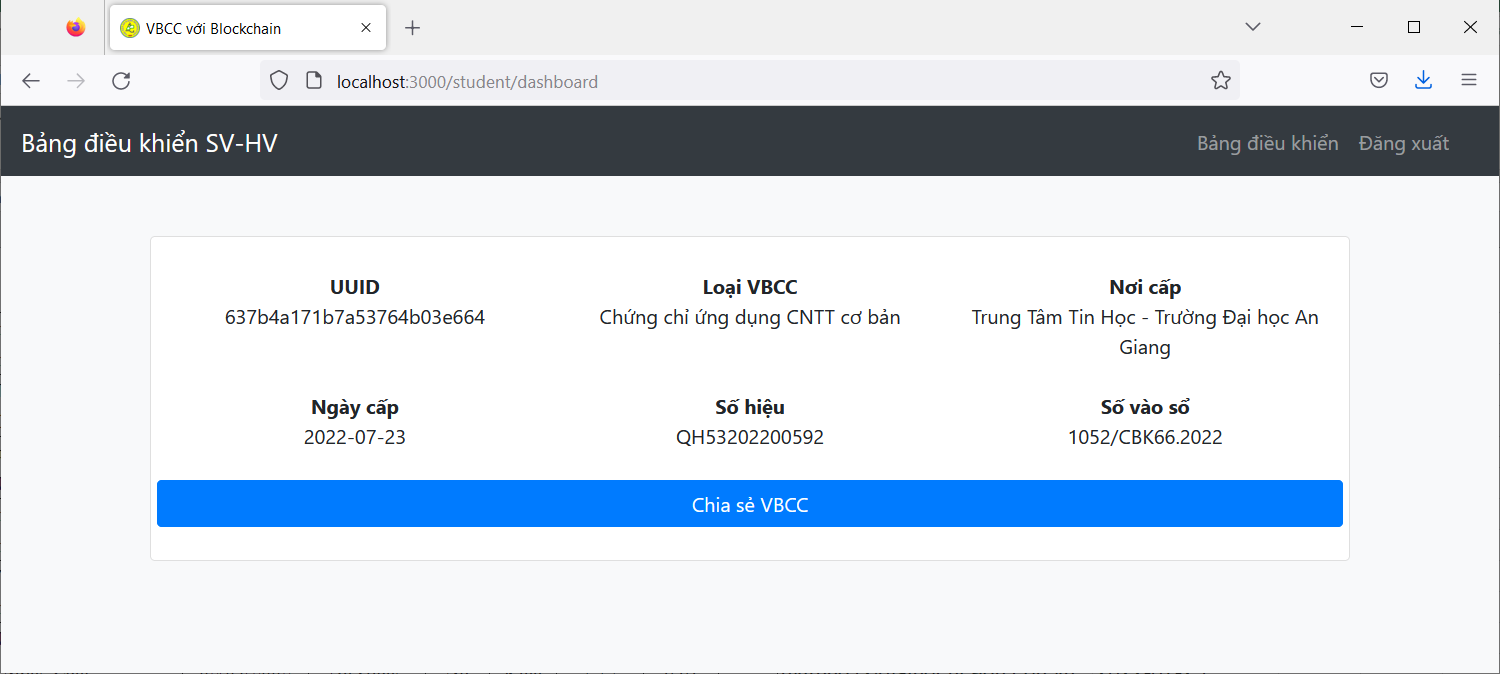
\includegraphics[width=.9\linewidth]{img/sv_hva.PNG}
\caption{Màn hình xem các VBCC đã nhận}
\label{fig:sv_hva}
\end{figure}

\begin{figure}[H]
\centering
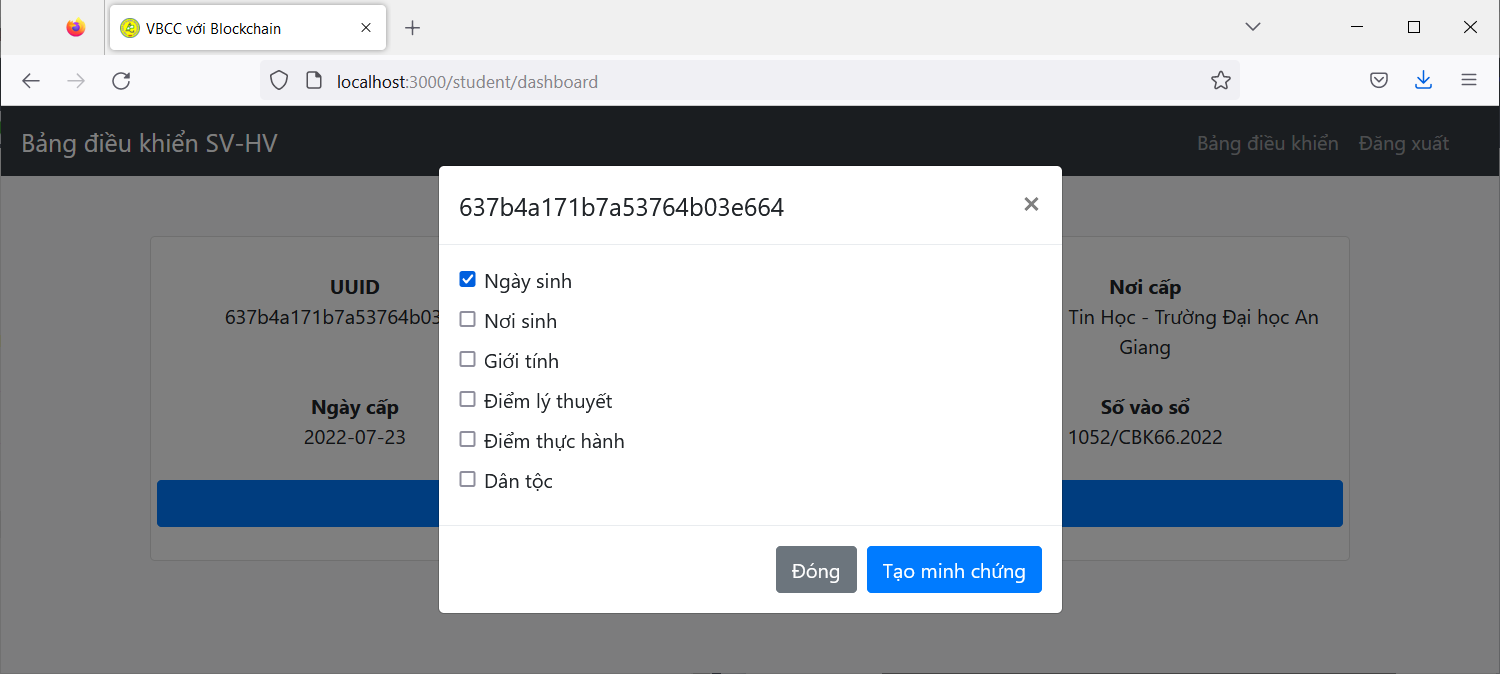
\includegraphics[width=.9\linewidth]{img/sv_chiase.PNG}
\caption{Màn hình chia sẻ thông tin VBCC}
\label{fig:sv_chiase}
\end{figure}

\begin{figure}[H]
\centering
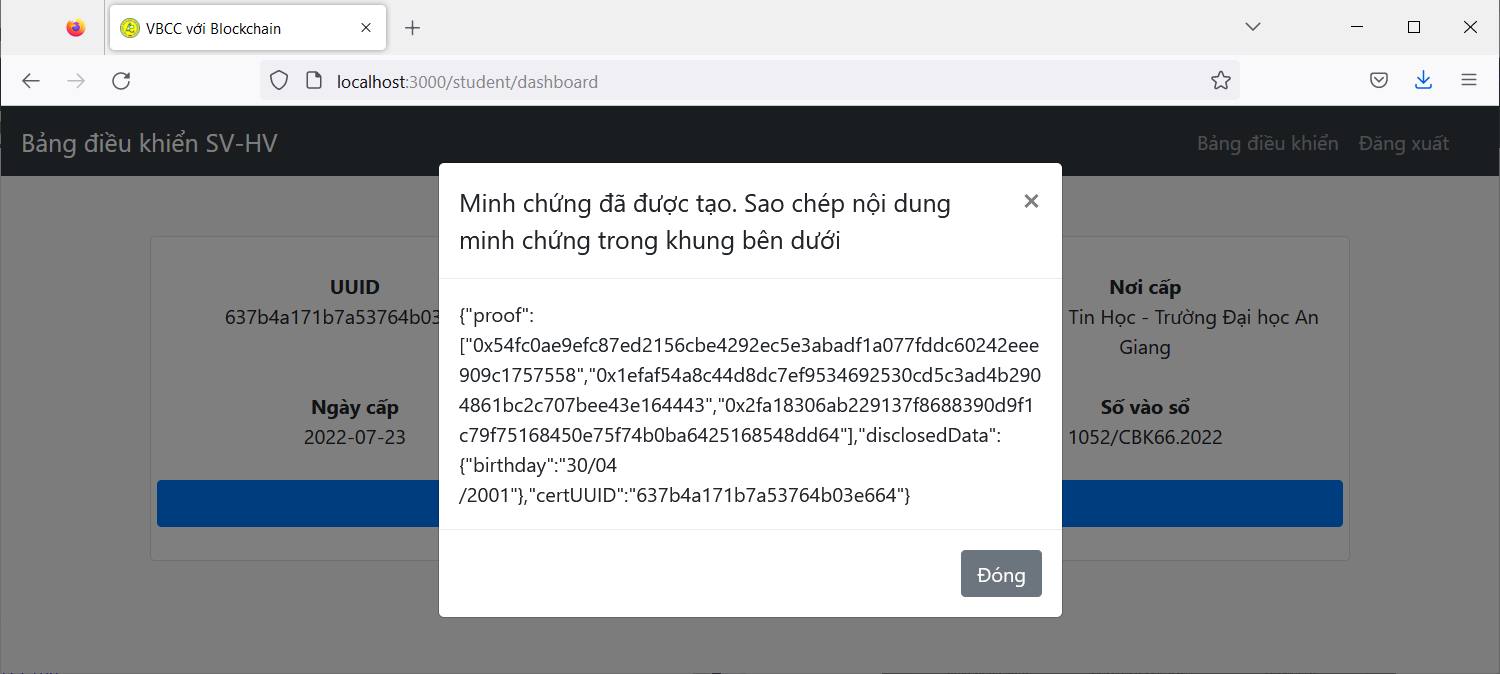
\includegraphics[width=.9\linewidth]{img/sv_minhchung.PNG}
\caption{Màn hình hiển thị mã xác thực VBCC}
\label{fig:sv_minhchung}
\end{figure}

Đơn vị xác minh chứng chỉ có chức năng

\begin{figure}[H]
\centering
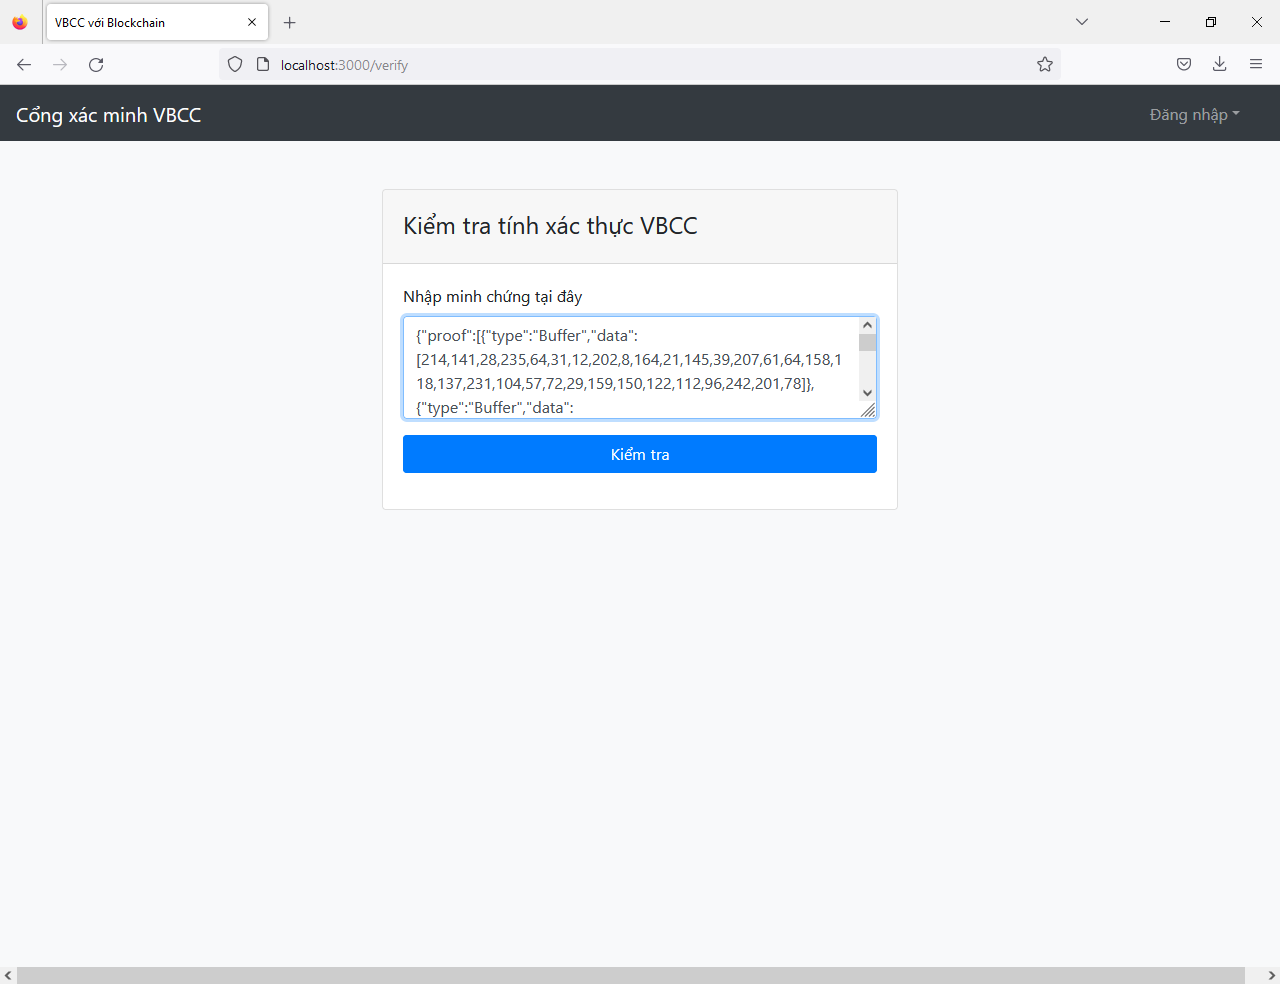
\includegraphics[width=.9\linewidth]{img/v_begin.PNG}
\caption{Màn hình nhập mã xác thực VBCC}
\label{fig:v_begin}
\end{figure}


